Having covered the importance of LLM optimization and the technical architecture of transformers in previous chapters, we now turn to the practical challenge of model compression.

This chapter begins with preliminary experiments on layer manipulation that revealed crucial insights about architectural redundancy in transformer models and shaped the main compression strategy. The chapter then presents what is possibly the heart of this research: a multi-stage pipeline that combines several optimization techniques in a structured sequence. Each stage is examined with both theoretical foundations and practical implementation details. Finally, the evaluation methods and their underlying motivation are detailed.

\section{Preliminary Research: Franken-LLaMA} \label{frankenllama}

Before embarking on systematic compression techniques for our target 1B parameter LLaMA model, we conducted preliminary research to understand the behavior of transformer architectures under structural modifications. This exploratory consisted on the ``Franken-LLaMA'' project \cite{franken-llama}, which involved experimenting with selective layer skipping and repetition in the larger LLaMA2-7B-Chat \cite{llama2} model to gain a first insight into which components of the transformer architecture are most critical for maintaining model performance.

The approach centered on modifying the standard transformer execution flow by selectively including, excluding, or repeating attention blocks within the 32-layer architecture. The repetition strategy was particularly attractive as it could theoretically reduce memory footprint by reusing the same layer weights multiple times rather than storing distinct parameters for each position. This weight sharing approach aligned directly with the target hardware constraints outlined in Section \ref{target_hardware}, where the memory limitation makes parameter reduction a critical optimization target.

25 different layer configurations were tested, each of which was evaluated through qualitative text generation tasks and quantitative assessment on the HellaSwag dataset \cite{hellaswag}.
The results revealed several that conservative modification, often maintained reasonable performance while reducing computational overhead. In particular, skipping the layers more towards the middle of the model rather than its ends resulted in low performance degradation. For instance, the configuration that skipped layers 23-27 achieved a HellaSwag score of 0.38 compared to the baseline's 0.34, suggesting that certain middle layers may contribute less to final performance than expected.

However, more aggressive modifications typically led to severe degradation in output quality. Configurations involving extensive layer repetition or using only sparse layer selections often produced incoherent text with non-ASCII characters and semantic breakdown. This behavior indicated that while some redundancy exists in the transformer architecture, maintaining a balanced representation across different depths remains crucial for coherent language generation.

These preliminary findings informed the subsequent approach to systematic compression: it revealed that strategic layer removal could sometimes improve performance metrics, suggesting that pruning techniques might offer promising avenues for optimization; at the same time, it showed how layer repetition was not a viable strategy and caused heavy performance degradation.

\section{An Overview of the Pipeline}

The core result of this research is the compression pipeline, which implements a sequential approach that combines multiple optimization techniques in a carefully orchestrated manner. As previously mentioned, the target model for these optimizations is LLaMA 3.2 1B, a distilled version of the larger LLaMA 3.2 model that has already undergone some level of pruning during its creation, according to the Hugging Face model documentation \cite{llama3_1b}.

The choice of this particular model as the starting point is both strategic and practical. While incorporating distillation directly into the pipeline would have been ideal given its effectiveness as a compression technique, the computational requirements make it rather prohibitive. Distillation essentially requires training a model from scratch, demanding extensive GPU resources that far exceed the computational budget available for the project. Thus, an existing pre-distilled model was utilized instead which already provides a compact yet capable foundation.

The pipeline follows a five-stage progression, with each stage building upon the previous one. The particular ordering was chosen based on the complementary nature of these techniques and their relative impact on model structure.

\begin{enumerate}
    \item The first stage implements depth-wise pruning (Section \ref{depth_pruning}), where entire transformer layers are removed based on importance metrics computed during a calibration phase. This coarse-grained approach eliminates redundant blocks, and ultimately redefines the skeleton of the architecture.

    \item Width-wise pruning follows as the second stage (Section \ref{wanda}), applying the WANDA algorithm to remove less critical weights within the remaining layers. This is a finer-grained approach compared to the depth-pruning, as it operates at the parameter level.

    \item The third stage introduces \textit{Low-Rank Adaptation} (LoRA) (Section \ref{lora}) to recover performance lost during the pruning phases, while also allowing for fine-tuning on specific downstream tasks.

    \item The fourth stage applies 4-bit quantization using GPTQ, reducing the memory footprint of individual parameters.

    \item The final stage includes an optional \textit{Eigenspace Low-Rank Approximation} (EoRA) step to improve the performance of the quantized model.
\end{enumerate}

Detailed descriptions of each stage are provided in the following sections. Each step yields an intermediate model suitable for independent evaluation, except when explicitly stated otherwise. The modular design supports selective execution through comprehensive tuning options, such as the ability to skip specific stages or experiment with different parameter configurations without modifying the core implementation. Having intermediate models allows to conduct ablation studies more easily and adapt the pipeline to specific hardware constraints.

\section{Depth-wise Pruning} \label{depth_pruning}

Depth pruning represents a structured approach to neural network compression that targets the architectural dimension of model depth rather than individual parameter elimination. Unlike width pruning, which reduces the size of weight matrices by removing neurons or attention heads while preserving the total number of layers, depth pruning removes entire layers or blocks from the network architecture. In the context of transformer-based language models, this typically involves eliminating complete attention blocks, each containing both a multi-head attention module and feed-forward network components. Figure \ref{fig:pruning_comparison} shows a visual comparison between the two pruning techniques.

\begin{figure}[htbp]
    \centering
    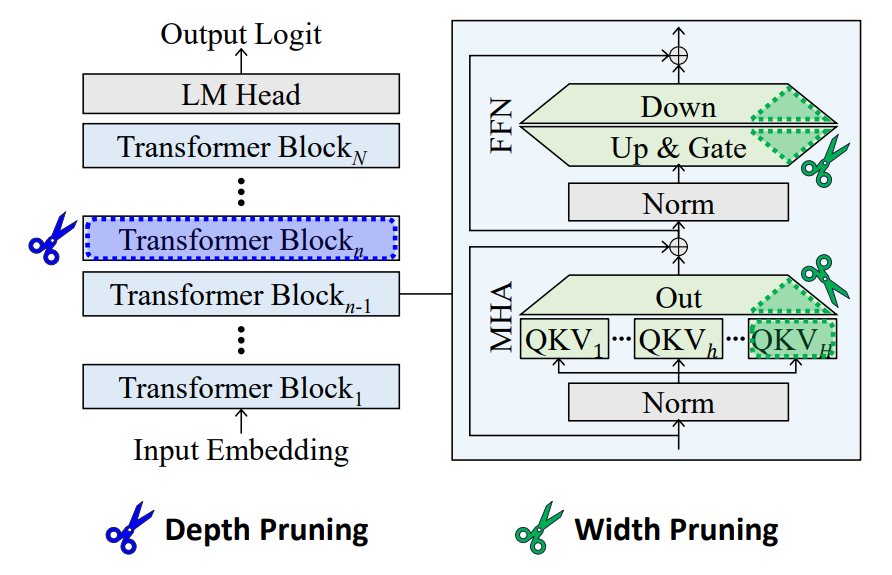
\includegraphics[width=0.7\textwidth]{pruning.png}
    \caption[Comparison of Depth and Width Pruning]{In depth pruning, we remove the single transformer layers (left). On the other hand, in width pruning we remove single neurons from the weight matrices (right). The image was sourced from \cite{shortened_llama}.}
    \label{fig:pruning_comparison}
\end{figure}

The depth pruning approach follows the methodology established by Kim et al. in their Shortened LLaMA work \cite{shortened_llama}, which demonstrated that removing entire transformer blocks can achieve competitive performance while delivering significant inference speedups, particularly under memory-constrained conditions. Rather than reducing individual weight dimensions as in width pruning, depth pruning eliminates entire layers from the model architecture, creating a more direct path to computational savings.

The depth pruning process begins with calculating layer importance scores using one of several metrics implemented in the pipeline. Three primary importance calculation methods are supported: magnitude-based scoring, Taylor expansion-based gradient analysis, and perplexity-based evaluation. The magnitude approach computes the L1 norm of weights within each transformer block, providing a simple baseline for layer significance. The Taylor method leverages first-order gradient information to estimate the impact of layer removal on model performance, following the approximation $L(W = 0) \approx L(W) + \nabla L \cdot (-W)$ where the gradient-weight product indicates layer importance. The perplexity method evaluates each layer by temporarily removing it and measuring the resulting degradation in language modeling performance on a calibration dataset.

Following the insights from Shortened LLaMA, the implementation protects the first four and last two layers from pruning, as these positions have been shown to be critical for maintaining performance (which is in line with what was discovered in Section \ref{frankenllama}). The remaining layers are ranked according to their importance scores, with the least significant layers selected for removal.

The removal process involves creating a new model architecture with the selected layers entirely eliminated, maintaining the original transformer structure for the remaining blocks. This approach contrasts sharply with width pruning techniques that create sparse weight matrices, as depth pruning produces models with clean, dense architectures that map naturally onto hardware accelerators without requiring specialized sparse computation support.

The implementation extends the Shortened LLaMA approach by integrating it into a comprehensive compression pipeline, where depth pruning serves as the foundation for subsequent optimization techniques. The layer importance calculations are performed efficiently using calibration datasets, typically requiring only 10 samples from standard corpora to produce reliable importance rankings. This efficiency makes depth pruning particularly attractive for resource-constrained scenarios where extensive calibration is impractical.

\section{Width-wise Pruning} \label{wanda}

Following depth-wise pruning, the second stage of the compression pipeline applies width-wise pruning. As mentioned in Section \ref{depth_pruning}, it operates at the parameter level, eliminating individual weights within the remaining layers to achieve fine-grained compression. Width pruning can be either:
\begin{itemize}
    \item \textbf{Unstructured}:
    \item \textbf{Structured}:
\end{itemize}

\subsection{WANDA Algorithm Overview}

WANDA introduces a novel pruning metric that combines weight magnitudes with input activation statistics to determine parameter importance. The core insight behind this approach stems from the observation that large language models exhibit emergent large magnitude features in their hidden states—outlier activations that are significantly larger than typical values and are crucial for model performance.

The WANDA importance metric for each weight $W_{ij}$ is defined as:

\begin{equation}
S_{ij} = |W_{ij}| \cdot \|X_j\|_2
\end{equation}

where $|W_{ij}|$ represents the absolute value of the weight and $\|X_j\|_2$ evaluates the L2 norm of the $j$-th input feature across all calibration samples. This formulation addresses a key limitation of traditional magnitude-based pruning: it fails to account for input activations, which play an equally important role in determining neuron outputs, especially in the presence of large magnitude features.

\subsection{Structured N:M Sparsity Implementation}

While WANDA was originally designed for unstructured sparsity, the compression pipeline implements its structured variant to leverage hardware acceleration capabilities. Specifically, the implementation focuses on structured N:M sparsity patterns, where at most N out of every M consecutive weights are non-zero.

The structured pruning process operates as follows:

\begin{enumerate}
   \item \textbf{Importance Calculation}: For each linear layer, compute the WANDA metric for all weights using calibration data
   \item \textbf{Grouping}: Organize weights into groups of M consecutive elements within each output channel
   \item \textbf{Selection}: Within each group, identify the N weights with the highest importance scores
   \item \textbf{Pruning}: Set the remaining (M-N) weights to zero
\end{enumerate}

This structured approach enables the use of specialized hardware accelerators, such as NVIDIA's sparse tensor cores, which can efficiently handle N:M sparsity patterns during inference.

\subsection{Implementation Details}

The WANDA implementation integrates seamlessly into the compression pipeline through the \texttt{prune\_wanda} function. Key implementation aspects include:

\textbf{Calibration Setup}: The algorithm uses the same calibration dataset as the depth pruning stage, typically consisting of 10 samples from the C4 corpus, ensuring consistency across optimization stages.

\textbf{Layer-wise Processing}: WANDA processes each transformer layer sequentially, updating activations after each layer is pruned to ensure that subsequent layers receive realistic input distributions.

\textbf{Per-output Comparison}: Following the original WANDA methodology, weights are compared and pruned on a per-output basis rather than globally across the layer. This approach maintains balanced pruning ratios across different output features, which proves crucial for preserving model performance.

\textbf{Binary Search for Sparsity}: For the variant implementation, a binary search algorithm finds the optimal threshold parameter $\alpha$ that achieves the target sparsity ratio while maximizing the cumulative importance of retained weights.

\subsection{Advantages and Computational Efficiency}

WANDA offers several advantages over more complex pruning methods:

\begin{itemize}
   \item \textbf{Single Forward Pass}: Unlike methods requiring iterative weight updates, WANDA completes pruning in a single forward pass through the model
   \item \textbf{No Weight Updates}: The algorithm requires no modifications to the remaining weights, suggesting that effective sparse subnetworks exist within the original model
   \item \textbf{Low Computational Overhead}: With $O(d^2)$ complexity compared to $O(d^3)$ for second-order methods, WANDA provides significant computational savings
   \item \textbf{Hardware Compatibility}: The structured N:M variant directly maps to accelerator capabilities without requiring specialized sparse computation libraries
\end{itemize}

The integration of WANDA as the width pruning stage creates a foundation for subsequent optimization techniques while maintaining the model's core functionality. The structured sparsity patterns ensure that the compressed model can benefit from hardware acceleration during inference, making this approach particularly suitable for deployment scenarios with strict performance requirements.
\section{LoRA} \label{lora}
\section{Quantization and EoRA} \label{quantization}
\section{Evaluation}